\documentclass[preprint,12pt]{elsarticle}
\usepackage{graphicx}
\usepackage[margin=1.0in]{geometry}
\usepackage{color, colortbl}
\usepackage{hyperref}
\usepackage{float}
% \usepackage[affil-it]{authblk}
\usepackage{subcaption}
\newcommand{\note}[1]{\textcolor{blue}{#1}}
\definecolor{LightCyan}{rgb}{0.88,1,1}
\definecolor{LightRose}{rgb}{1,0.88,0.88}
\definecolor{LightGreen}{rgb}{0.88,1,0.88}

\title{Real-Time event reconstruction for Nuclear Physics Experiments using Artificial Intelligence}
\author[1]{Gagik Gavalian}

\address[1]{Jefferson Lab, Newport News, VA, USA}
%\address[2]{CRTC, Department of Computer Science, Old Dominion University, Norfolk, VA, USA}
%Authored by Jefferson Science Associates, LLC under U.S. DOE Contract No. DE-AC05-06OR23177. The U.S. Government retains a non-exclusive, paid-up, irrevocable, world-wide license to publish or reproduce this manuscript for U.S. Government purposes.

%\fntext[fn1]{Authors contributed equally.}
%\fntext[fn2]{Correspoding author, \textit{gavalian@jlab.org}}


\begin{document}

%\begin{titlepage}

\begin{abstract}
\indent
Charged track reconstruction is a critical task in nuclear physics experiments, enabling the identification and analysis of particles produced in high-energy collisions. Machine learning (ML) has emerged as a powerful tool for this purpose, addressing the challenges posed by complex detector geometries, high event multiplicities, and noisy data. Traditional methods rely on pattern recognition algorithms like the Kalman filter, but ML techniques, such as neural networks, graph neural networks (GNNs), and recurrent neural networks (RNNs), offer improved accuracy and scalability. By learning from simulated and real detector data, ML models can identify and classify tracks, predict trajectories, and handle ambiguities caused by overlapping or missing hits. Moreover, ML-based approaches can process data in near-real-time, enhancing the efficiency of experiments at large-scale facilities like the Large Hadron Collider (LHC) and Jefferson Lab (JLAB). As detector technologies and computational resources evolve, ML-driven charged track reconstruction continues to push the boundaries of precision and discovery in nuclear physics. 

In this talk, we highlight advancements in charged track identification leveraging Artificial Intelligence within the CLAS12 detector, achieving a notable enhancement in experimental statistics compared to traditional methods. Additionally, we showcase real-time event reconstruction capabilities, including the inference of charged particle properties such as momentum, direction, and species identification, at speeds matching data acquisition rates. These innovations enable the extraction of physics observables directly from the experiment in real-time.
\end{abstract}
%\end{titlepage}
\maketitle

\section{Introduction}
\indent
Nuclear physics experiments have grown increasingly complex over recent decades, featuring more sophisticated detector systems and higher luminosities. In new experiments with elevated detector occupancies, innovative approaches to data processing are essential to enhance both the accuracy and speed of data reconstruction. Advances in Artificial Intelligence (AI) offer promising alternatives to traditional algorithms, with Machine Learning (ML) techniques being utilized at various stages of experimental data processing, including detector reconstruction, particle identification, detector simulations, and physics analysis.

This paper explores the integration of machine learning models into the CLAS12 charged-particle track reconstruction software. It provides a comprehensive analysis of the reconstruction performance, highlighting improvements in track reconstruction efficiency and processing speed compared to conventional methods.


\section{CLAS12 Detector}

The CLAS12 (CEBAF Large Acceptance Spectrometer for 12 GeV) detector is a state-of-the-art experimental apparatus used in nuclear physics research. It is located at the Thomas Jefferson National Accelerator Facility (Jefferson Lab) in Newport News, Virginia. The detector is part of an upgrade to the Continuous Electron Beam Accelerator Facility (CEBAF), which increased the maximum energy of the electron beam from 6 GeV to 12 GeV. This upgrade allows for a more in-depth exploration of the structure and properties of nucleons (protons and neutrons) and the nature of the strong force that binds them together in the atomic nucleus.

\begin{figure}[h!]
\centering
\centerline{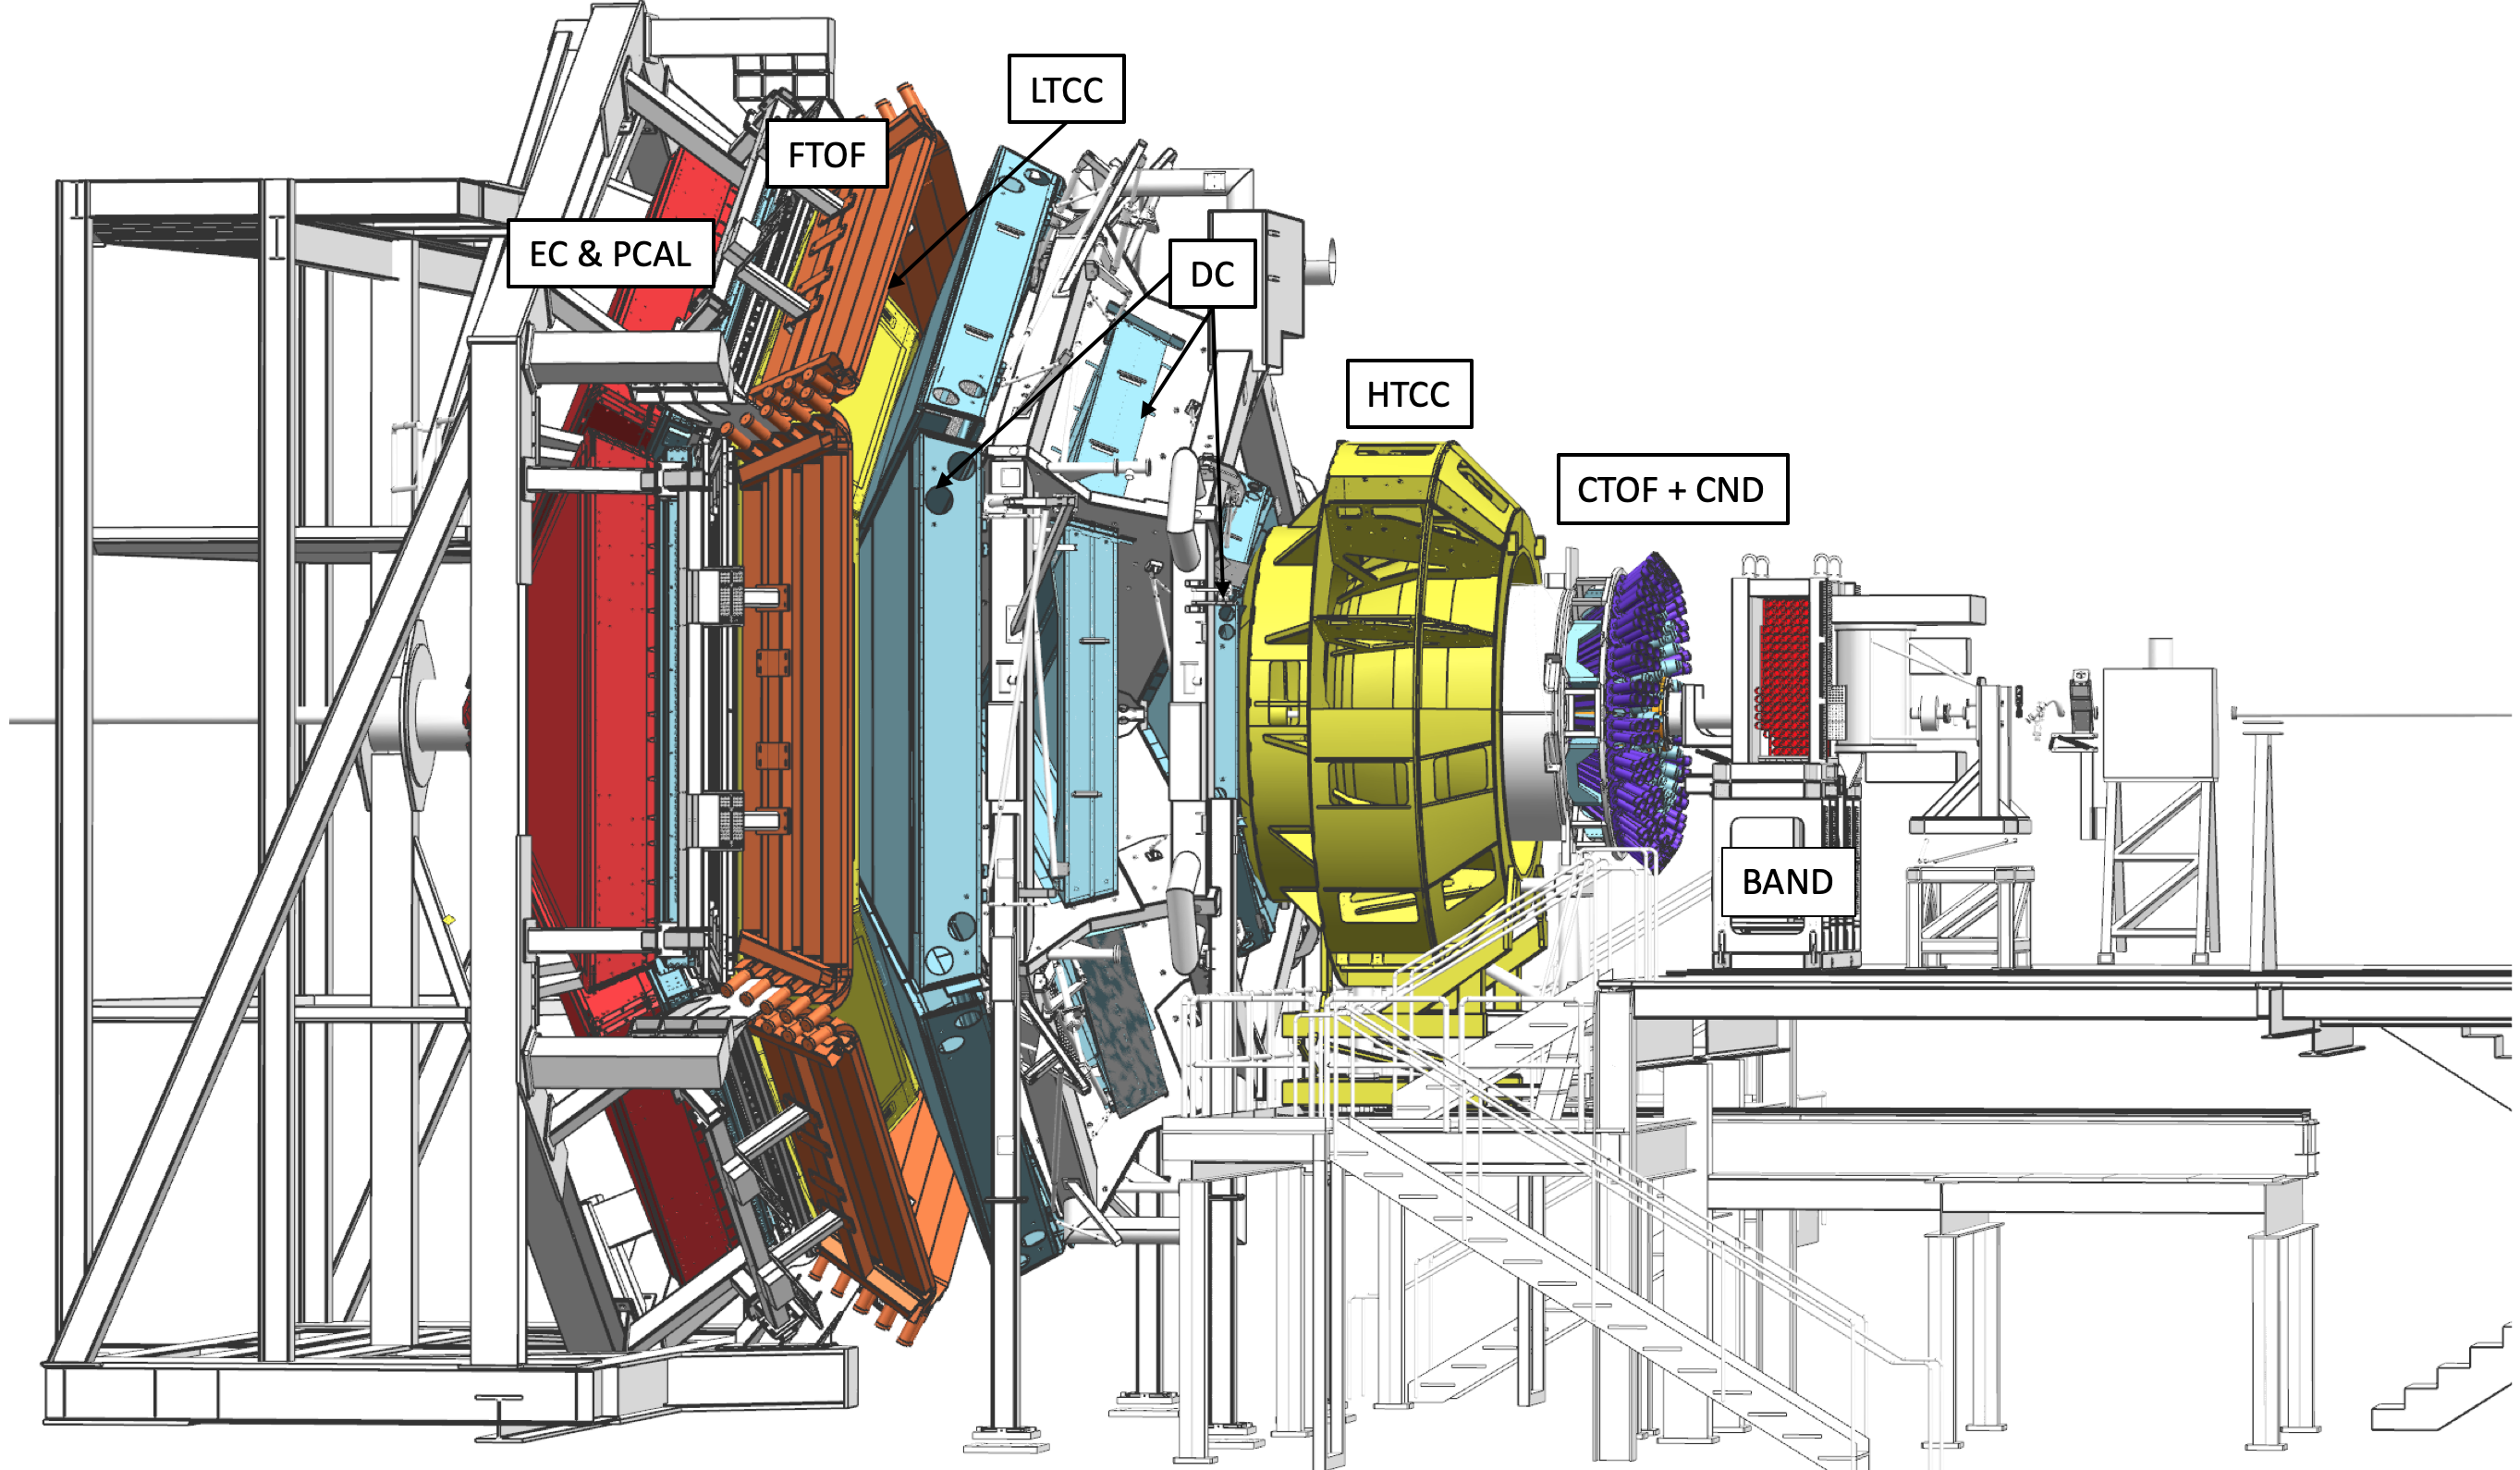
\includegraphics[width=0.7\columnwidth]{images/CLAS12-side.png}}
\caption{The CLAS12 detector in the Hall~B beamline. The electron beam enters from the right and impinges on
  the production target located in the center of the solenoid magnet shown at the right (upstream) end of CLAS12,
  where other detector components are also visible. Scattered electrons and forward-going particles are detected
  in the Forward Detector (FD), consisting of the High Threshold Cherenkov Counter (HTCC) (yellow), 
  followed by the torus magnet (gray), the drift chamber tracking system (light blue),
  and time-of-flight scintillation counters (brown), and electromagnetic calorimeters (red). } 
\label{fig:CLAS12}
\end{figure}

Key features and capabilities of the CLAS12 detector include:

\begin{itemize}

\item{\bf Large Acceptance: } As its name suggests, CLAS12 has a large angular and momentum acceptance. This feature is crucial for detecting particles over a wide range of angles and energies, allowing comprehensive analysis of nuclear reactions.
\item{\bf Electron Beam Experiments:} CLAS12 is designed to investigate the interactions of high-energy electrons with nucleons and nuclei. By scattering electrons off target materials, scientists can probe the internal structure of nucleons and the dynamics of the strong force.
\item{\bf High Luminosity:} The detector operates at high luminosities, enabling it to collect a vast amount of data from electron scattering experiments. This high data rate is essential for studying rare processes and achieving statistically significant results.
\item{\bf Sophisticated Detection Systems:} CLAS12 consists of various subsystems designed to detect different types of particles and measure their properties. These include drift chambers for tracking charged particles, time-of-flight counters for particle identification, calorimeters for measuring energy, and Cherenkov detectors for identifying electrons.
\item{\bf Versatility:} The detector is versatile and can be used for a wide range of experiments, from studying the quark-gluon structure of nucleons to investigating the properties of nuclei under extreme conditions.
\item{\bf Data Analysis and Simulation:} Advanced software and computational tools are used to analyze the data collected by CLAS12. These tools include simulation packages that model the detector's response and data analysis frameworks for extracting physical quantities from the experimental data.
\end{itemize}
In summary, CLAS12 is a critical tool in modern nuclear physics, enabling researchers to delve deeper into the quantum world of nucleons and nuclei. Its advanced technology and capabilities contribute significantly to our understanding of fundamental physics, particularly in the realm of quantum chromodynamics (QCD), the theory describing the strong interaction.


\section{Drift Chamber Particle Tracking}

The CLAS12~\cite{Burkert:2020akg} forward detector is built around a six-coil toroidal magnet 
which divides the active detection area into six azimuthal regions, called ``sectors''. Each sector is 
equipped with three regions of drift chambers~\cite{Mestayer:2020saf} designed to detect charged 
particles produced by the interaction of an electron beam with a target. Each region consists of two 
chambers (called super-layers), each of them having six layers of wires. Each layer  in a super-layer 
contains 112 signal wires, making a super-layer a $6\times112$ cell matrix. 
The schematic view of all sectors and super-layers is shown in Figure~\ref{fig:drift_chambers}.

\begin{figure}[h!]
\centering
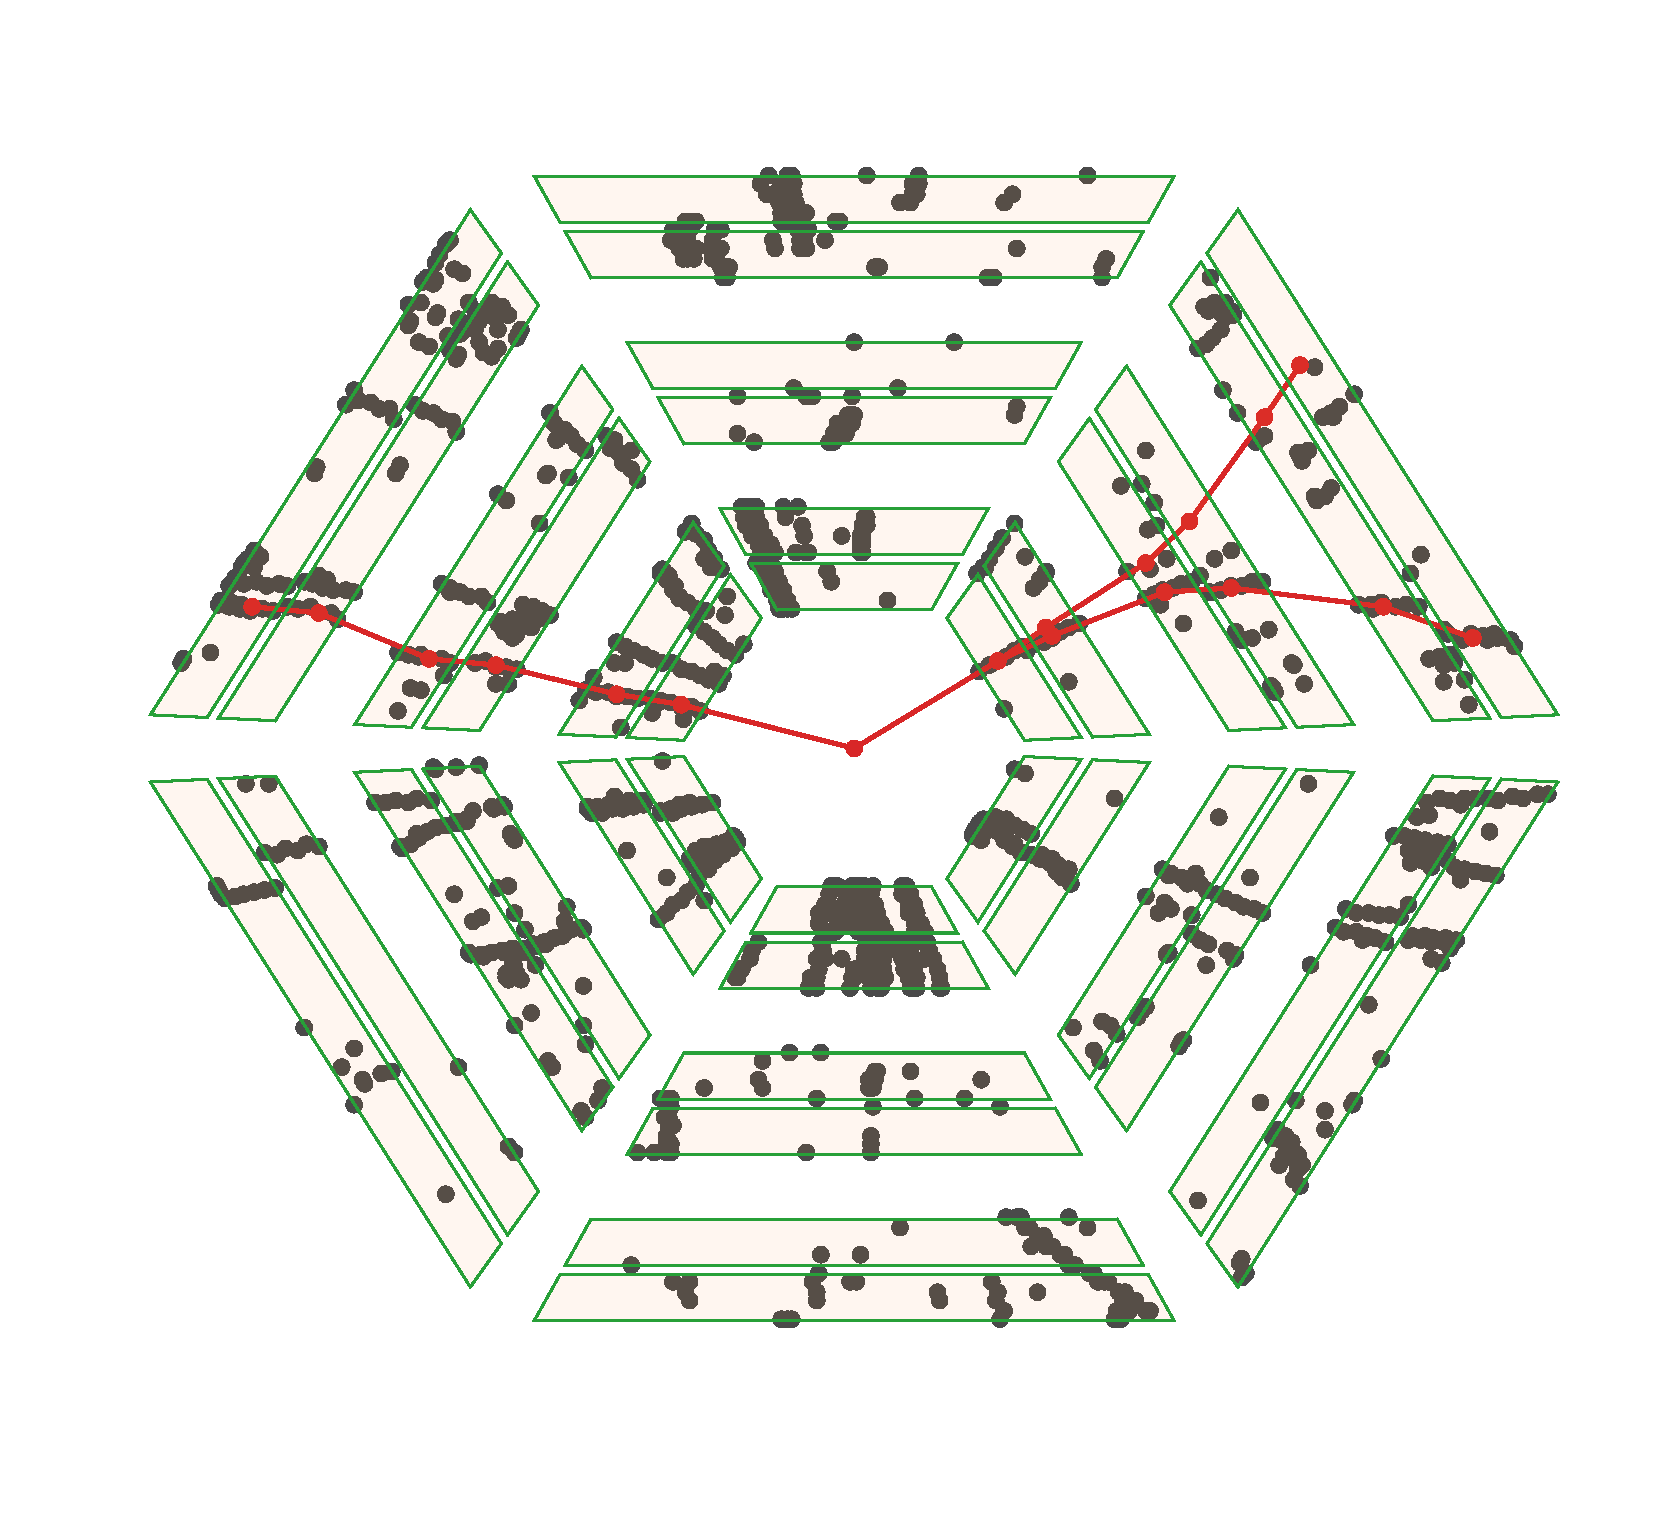
\includegraphics[width=0.32\columnwidth]{images/evt_05.pdf}
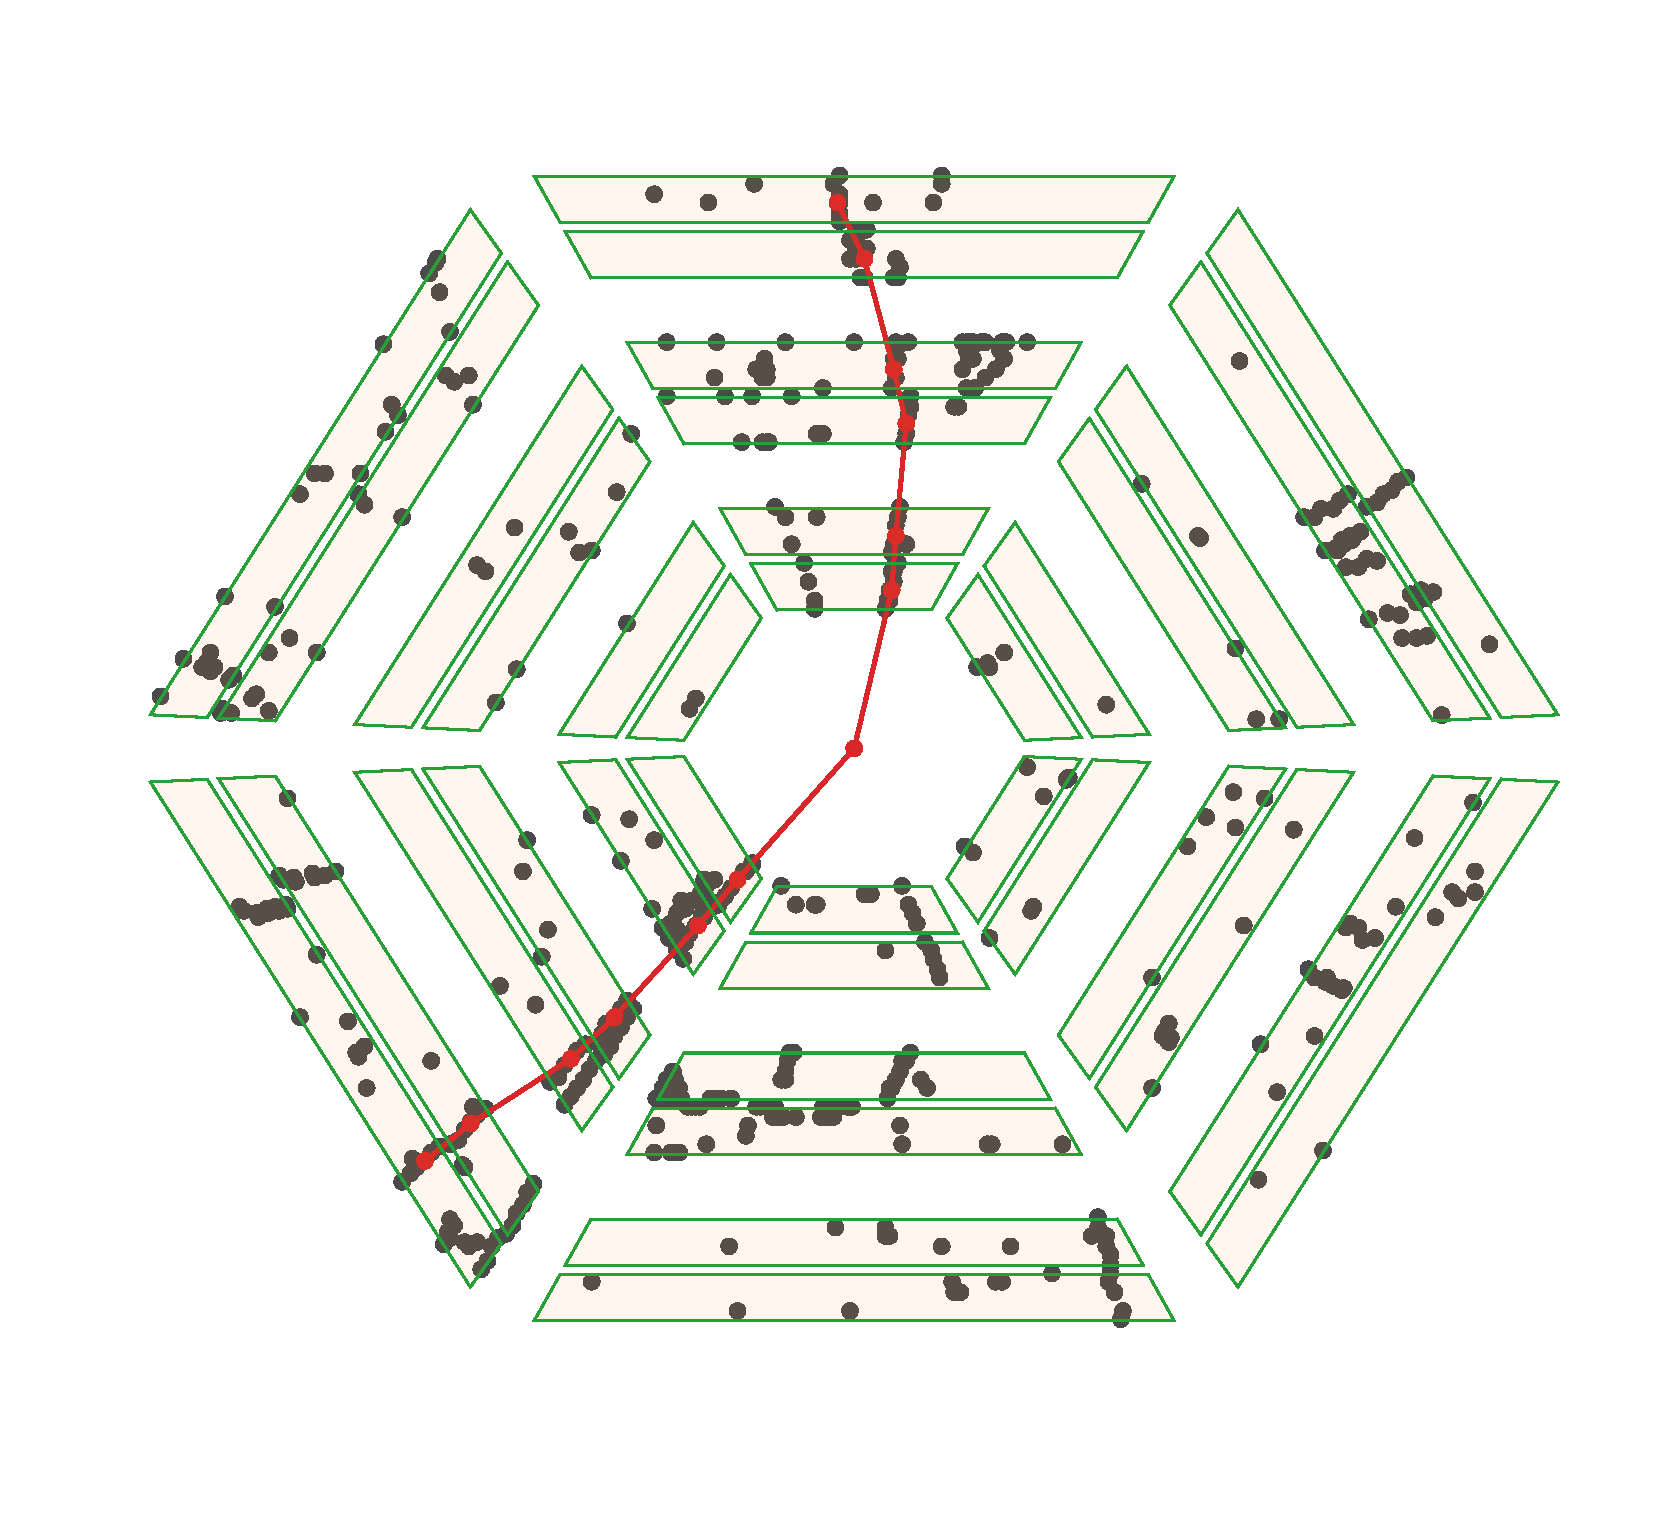
\includegraphics[width=0.32\columnwidth]{images/evt_26.pdf}
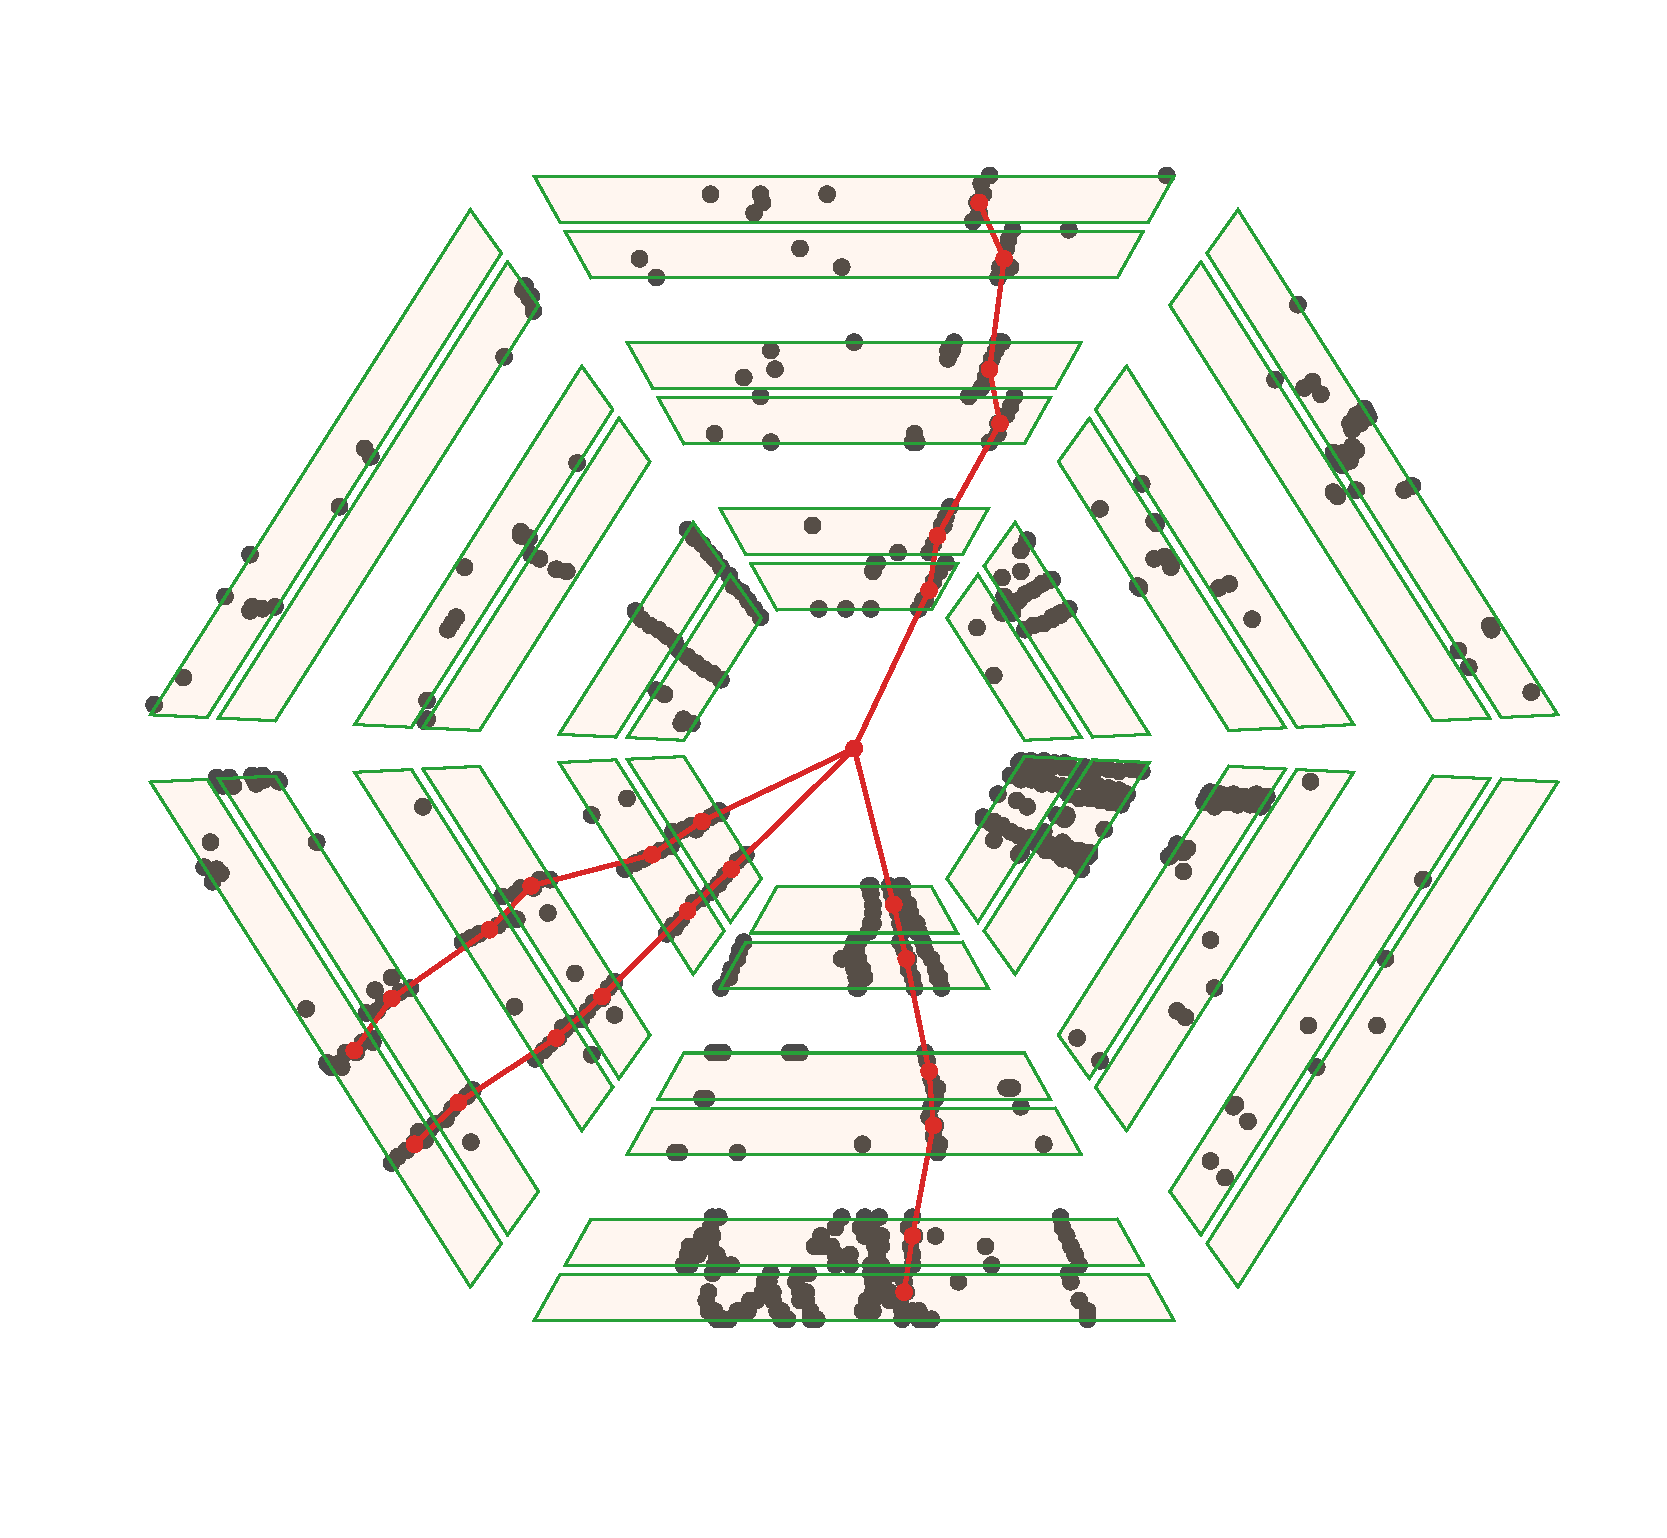
\includegraphics[width=0.32\columnwidth]{images/evt_35.pdf}
\caption{Example views of the six sectors of the Drift Chambers of CLAS12. The points show wire hits for each of the layers in the drift chambers and the lines indicate reconstructed tracks by the conventional CLAS12 tracking algorithm. } 
\label{fig:drift_chambers}
\end{figure}

Particles that originate from the interaction vertex travel through the magnetic field and pass through all 
three regions of the drift chambers in a given sector and are reconstructed by tracking algorithms. First, 
in each super-layer adjacent wires with a signal are grouped into segments. Track candidates are constructed 
by connecting segments in each super-layer to form a track trajectory. Then each track candidate is fitted through 
a magnetic field to calculate the quality of the track ($\chi^2$), and the track candidates with $\chi^2$ below the cut value
are saved for further refinement using Kalman-filter~\cite{Kalman1960}.

The positions of these segments in each super-layer are used to fit the track trajectory 
to derive initial parameters, such as momentum and direction (called "hit-based" tracking).  After the initial selection, good track candidates 
(shown in Figure~\ref{fig:drift_chambers} with lines) are passed through a Kalman-filter to 
refine measured parameters further (called "time-based" tracking).

%At the first stage of the tracking, the tracks are identified using only the hit positions (wire number). The precision 
%of the reconstructed track parameters using only hit positions are worse ($\sim3\%$) than the final calculated parameters from time-based tracking, but they are sufficient to calculate physics quantities from the event and identify desired reactions in the event. 

\begin{figure}[h!]
\centering
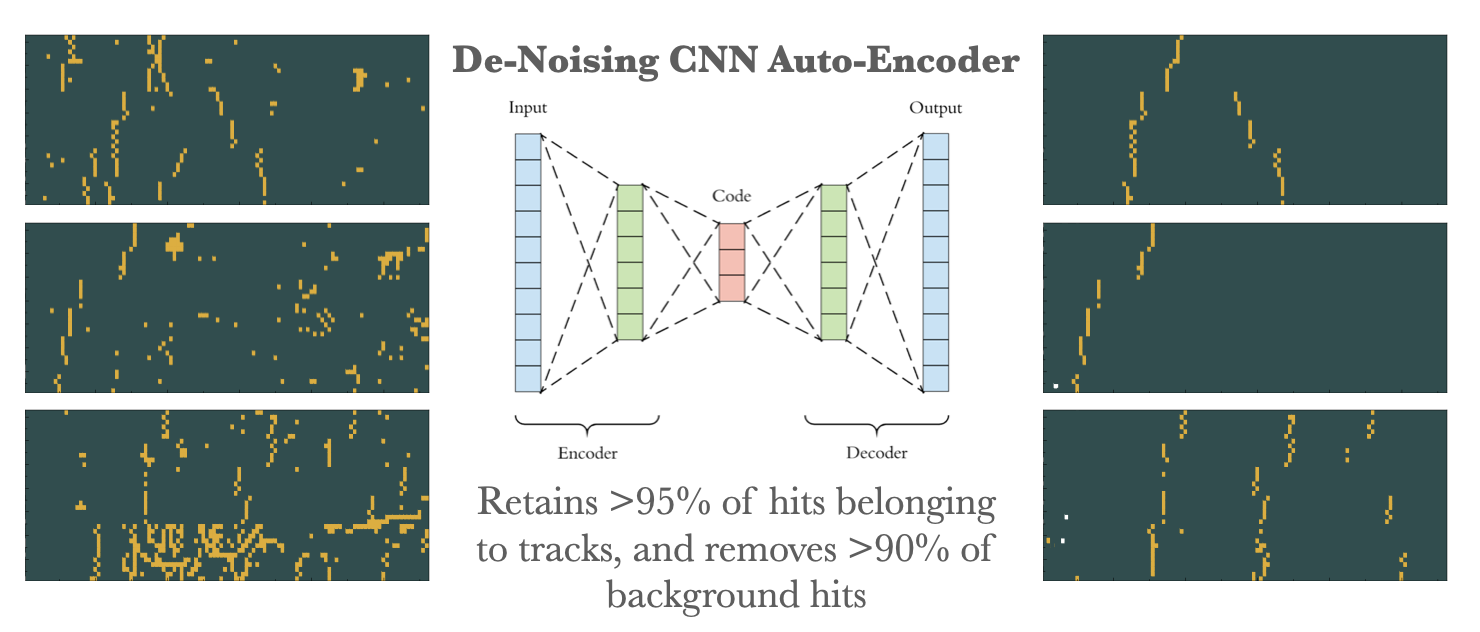
\includegraphics[width=0.85\columnwidth]{images/denoise_autoencoder.png}
\caption{Convolutional Auto-Encoder (CAE) trained on real data can efficiently remove noise hits from raw Drift Chmaber hits, leaving only hits potentially associated with tracks. } 
\label{fig:denoising}
\end{figure}

The CLAS12 track reconstruction process is already using AI at different stages of data reconstruction. First, a Convolutional
Autoencoder is used to de-noise the drift chamber hits~\cite{Thomadakis:2022zcd}, which leads to an improved cluster
identification in each super-layer. Examples of raw and denoised drift chamber hist are shown in Figure~\ref{fig:denoising},
where the network was trained on experimental data, providing the raw hits in drift chambers as an image of 36x112 as input and
the hits belonging to a reconstructed track as an output image. The Autoencoder learns to remove the noise hits, leaving only 
hits that can potentially form a track. After the denoising, a clustering algorithm finds segments in each superlayer to 
pass to the track-finding algorithm.

Then after the segment finding, the track candidate list is composed from all sensible combinations of segments in each super-layer.
These track candidates are then identified using a Multi-Layer Perceptron (MLP) classifier,
which identifies 6-super-layer and 5-super-layer track candidates~\cite{Gavalian:2020oxg}. Shown in Figure~\ref{fig:trackfinder} is 
the architecture of the network and tracks selected by the network from possible track candidates in one sector.

\begin{figure}[h!]
\centering
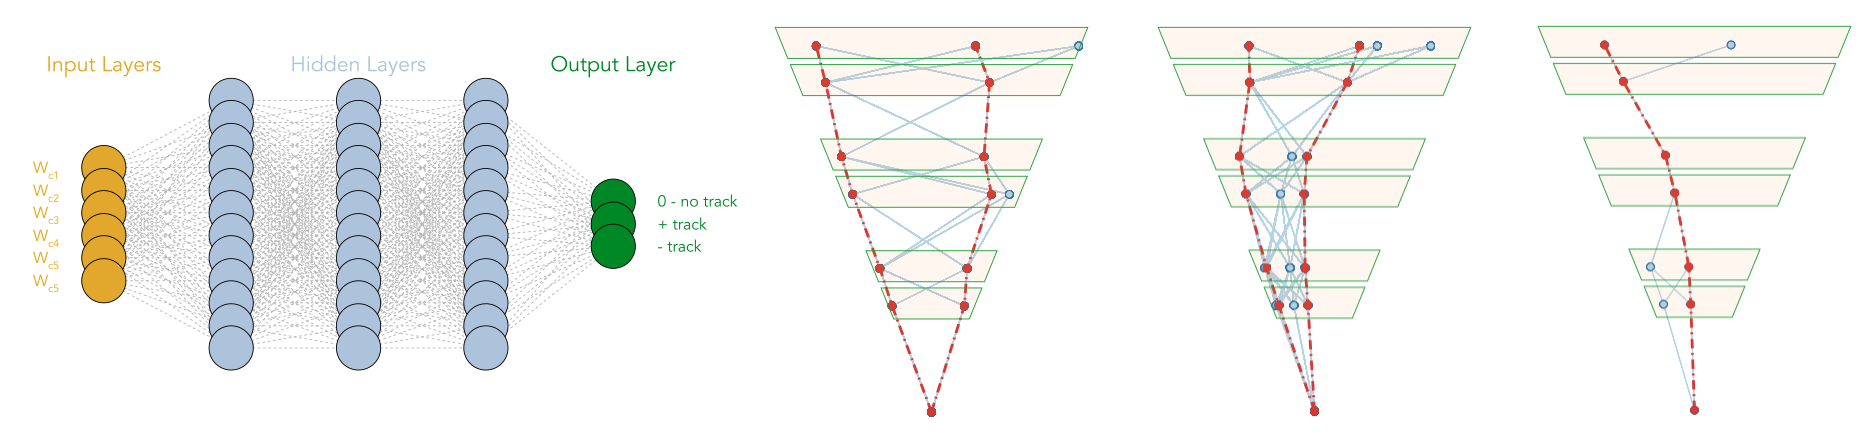
\includegraphics[width=0.85\columnwidth]{images/track_finder.png}
\caption{Multi-Layer Perceptron (MLP) network is used to identify tracks from combinations of segments measured in each super-layer of Drift Chambers. The input is a vector
of 6 numbers (average segment position in each super-layer, and the output is a vector of probabilities (3 labels), of false track, negatively charged track, and positively charged track. } 
\label{fig:trackfinder}
\end{figure}
The combination of de-noising and AI-assisted track candidate identification in CLAS12 results in a $50\%–75\%$ increase in statistics for multi-particle final states, depending on the kinematics and the number of detected particles in the final state~\cite{Gavalian:2020xmc}. Figure~\ref{fig:ai_vs_conv}(a) illustrates the analysis of the reaction $ep\rightarrow e^\prime\pi^+\pi^-(X)$ , comparing three different reconstruction workflows. The missing mass of the three detected particles is shown, with the missing proton peak clearly visible.

The "Conventional" workflow represents the standard reconstruction process without AI assistance. In the "AI-Assisted" workflow, the conventional procedure is augmented with track candidate predictions provided by the AI track classifier, yielding an approximate $30\%$ improvement in statistics. The "Denoised/AI-Assisted" workflow utilizes denoised drift chamber 
data to identify segments, which are then processed by the AI to suggest track candidates for the conventional track fitting algorithm. This workflow achieves a statistical increase of approximately $60\%$ in the missing mass distribution (for this particular reaction).

%The combined result of de-noising and AI-assisted track candidate identification used in CLAS12 leads to an increase in statistics of multi-particle final states of 
%$50\%-75\%$ depending on kinematics and number of detected particles in the final state~\cite{Gavalian:2020xmc}. In Figure~\ref{fig:ai_vs_conv} (a) analysis of a reaction $ep\rightarrow e^\prime\pi^+\pi^-(X)$ are 
%shown for three different reconstruction workflows. The missing mass of three detected particles in the event is shown with the missing proton peak visible.
%The "Conventional" workflow refers to a standard reconstruction procedure without any assistance from the Artificial 
%Intelligence. In the "AI-Assisted" workflow the conventional reconstruction procedure uses track candidate predictions suggested by AI track classifier and
%yields $\approx 30\%$ improvement in statistics. The "Denoised/AI-Assisted" workflow uses the denoised drift chamber data to find segments in the drift chambers,
%then uses AI to find and track candidates to be processed by conventional track fitting algorithm. This yields a statistical increase of $\approx 60\%$ in the missing mass 
%distribution.

%The developed AI tools for CLAS12 reconstruction can identify tracks from their cluster pattern and estimate the track parameters.
%If combined with the clustering algorithm, this chain may provide a complete track reconstruction solely based on AI algorithms and
%may potentially be used in real-time with data acquisition. 
%\section{Introduction}

During past few years there was a big interest in using Artificial Intelligence (AI) in 
various ares of nuclear physics, from data processing to physics analysis. With continuously 
improving methods of Machine Learning (ML) and computational hardware it becomes easy to 
substitute some computational tasks with ML algorithms leading to smaller and computationally
more efficient code base. In this article we discuss implementation of Convolutional Auto-Encoders 
for de-noising data from CLAS12~\cite{Burkert:2020akg} tracking detectors (Drift 
Chambers~\cite{Mestayer:2020saf}). The de-nosing was used to analyze simulated data to measure
improvement on track reconstruction efficiency.

%\section{Calorimeter}

A primary goal of the CLAS12 physics program is to study internal dynamics of the nucleon . 
These experiments require accurate kinematical analysis of neutral and charged particles at high momentum. 
In particular, all CLAS12 electro-production experiments require the efficient detection and reliable identification 
of energetic electrons, photons, and neutrons using the forward electromagnetic calorimeter (ECAL).

One of the primary usages of ECAL system is separating electrons from other particles, like pions, using 
energy deposited in the calorimeters. To accommodate hexagonal design of CLAS12 detector ECAL is using 
triangular hodoscope layout. The scintillating layers have three alternating stereo readout planes named U,V and W, 
which are interleaved with layers of lead as shown on Figure~\ref{clas12:ecal}

\begin{figure}[!ht]
\begin{center}
 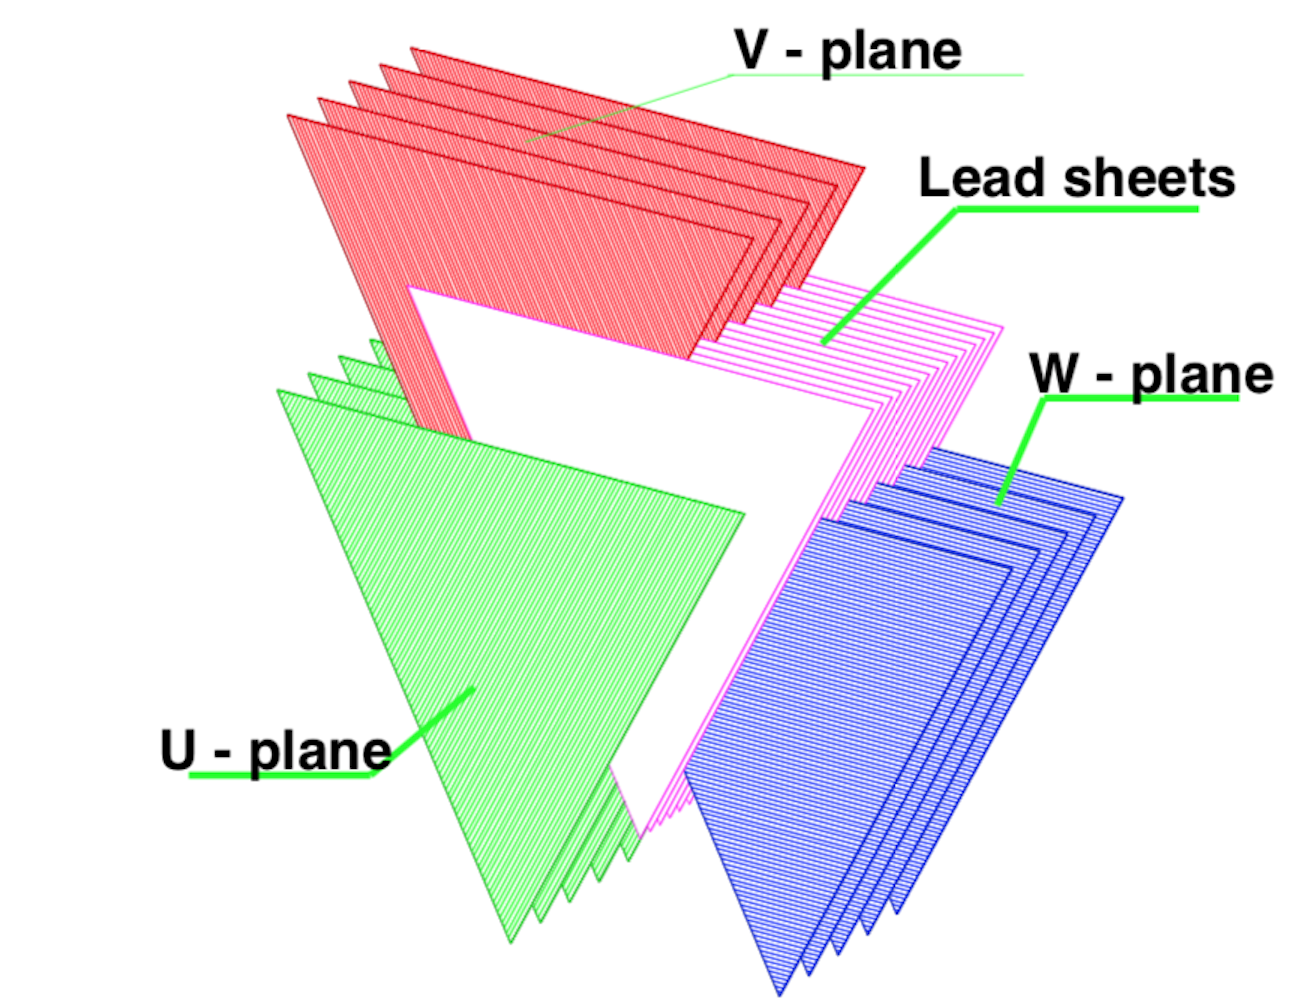
\includegraphics[width=3.in]{images/calorimeter_layers.png}
 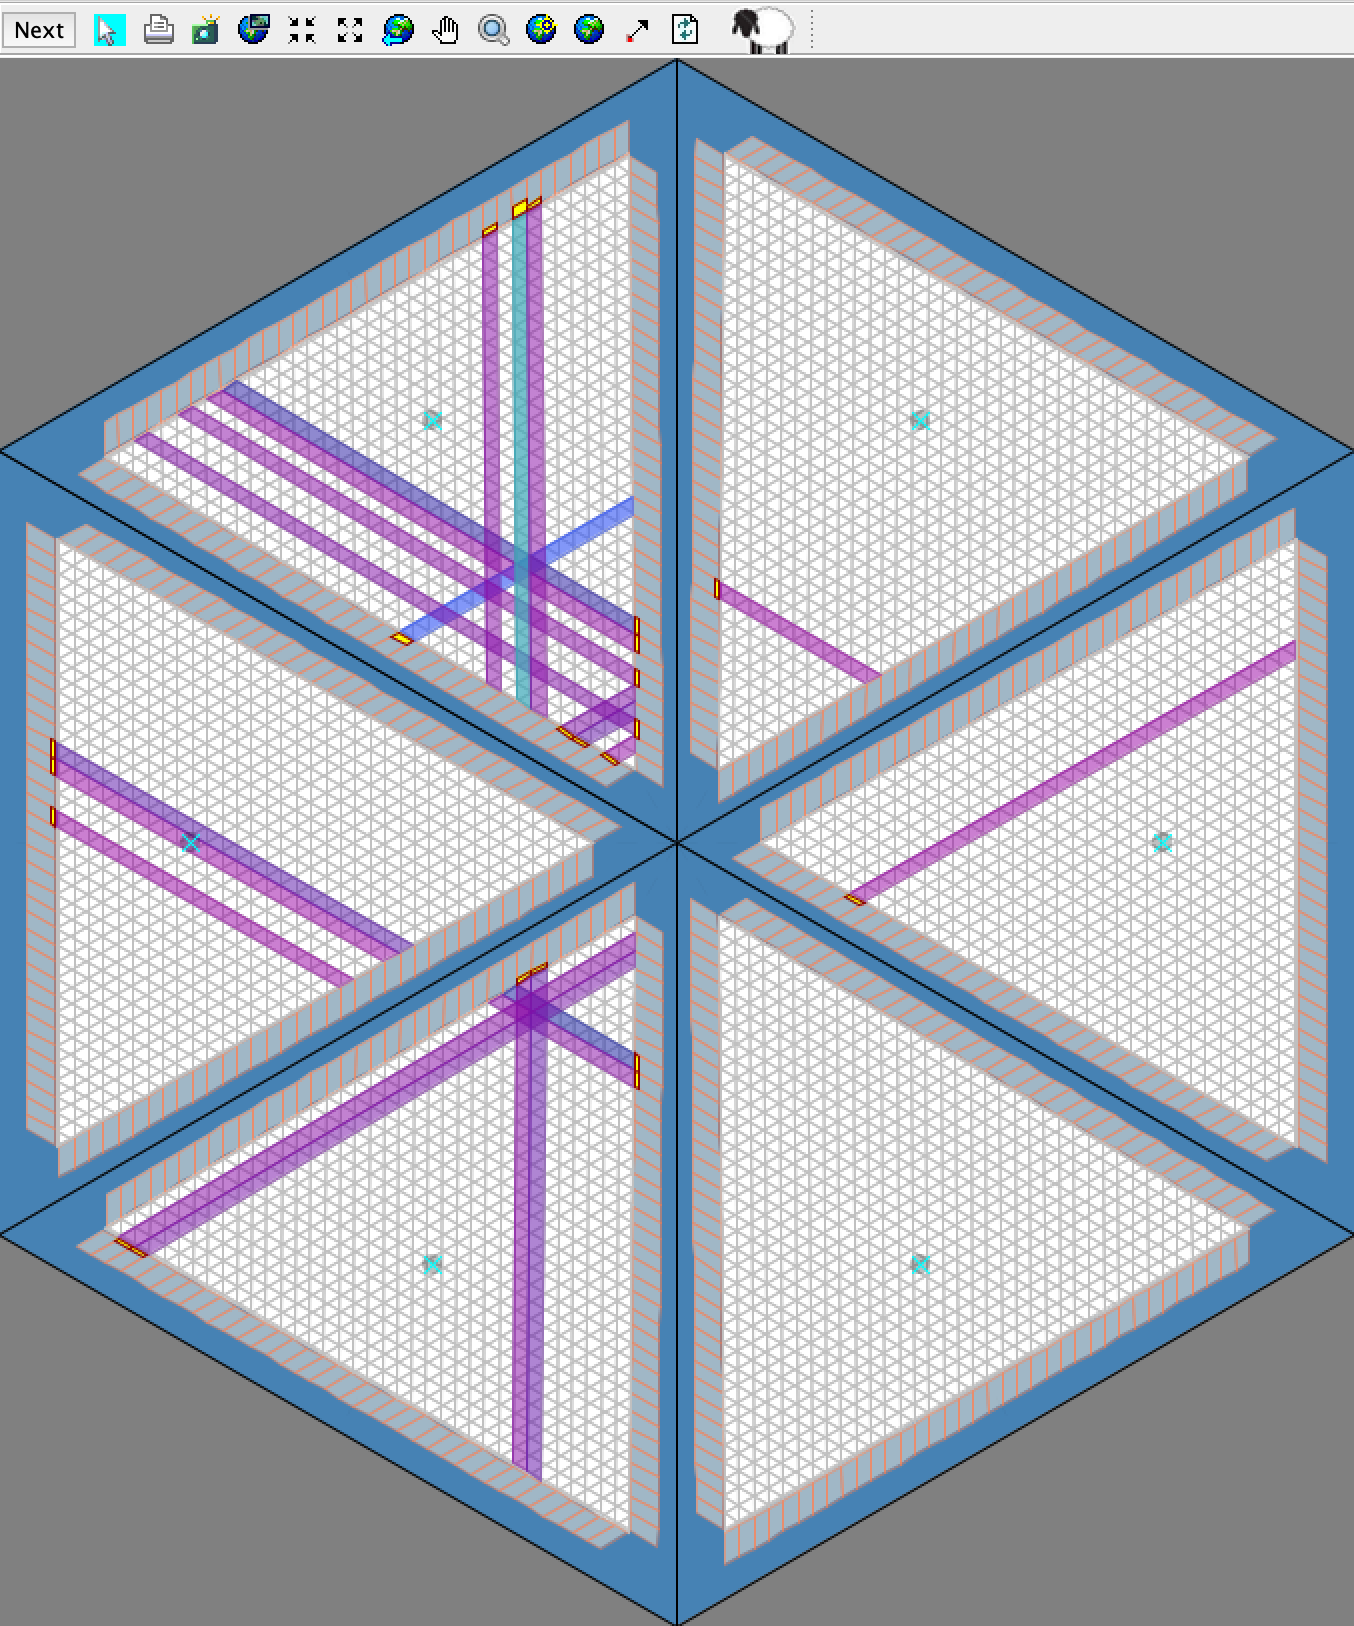
\includegraphics[width=2in]{images/ecal_view.png}
\caption { CLAS12 Electromagnetic Calorimeter structure description.}
 \label{clas12:ecal}
 \end{center}
\end{figure}

When particle enters the calorimeter it leaves signal in each of the layers (U,V and W), and is readout independently.
For each layer a cluster (called peak) is constructed by grouping adjacent hit strips and peaks from all three sides are combined into a cluster if they intersect in one point on the surface. A typical cluster is shown on Figure~\ref{clas12:ecal}.


\begin{figure}[h!]
\centering
%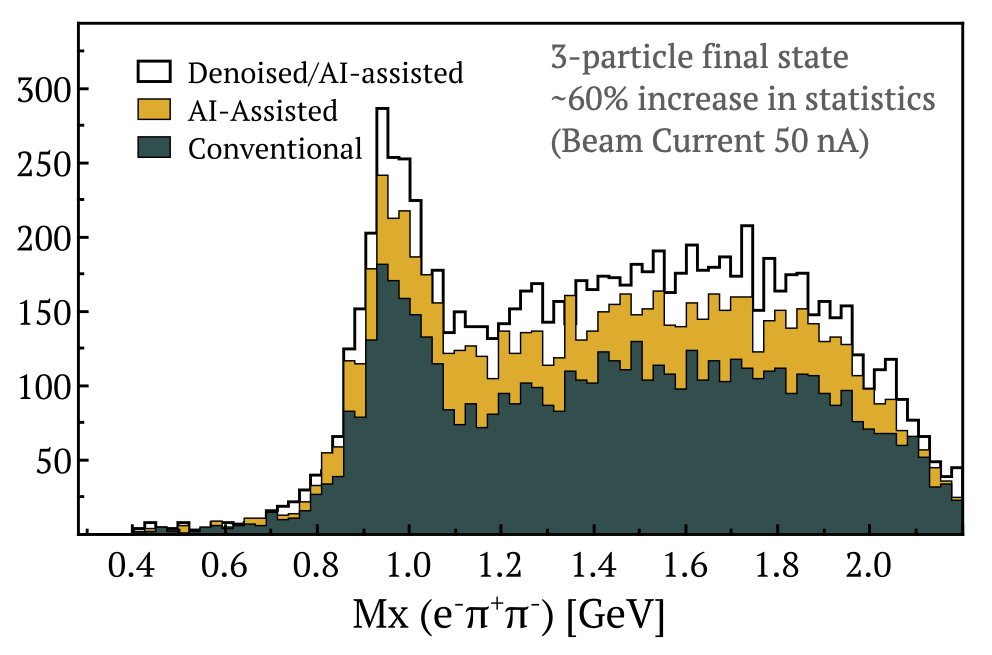
\includegraphics[width=0.45\columnwidth]{images/ai_vs_conv_tracking.png}
%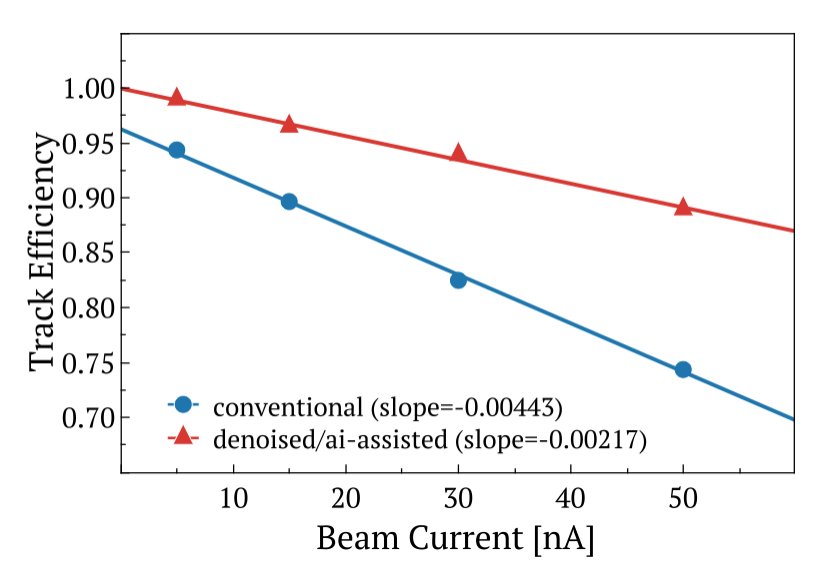
\includegraphics[width=0.44\columnwidth]{images/lumi_scan.png}
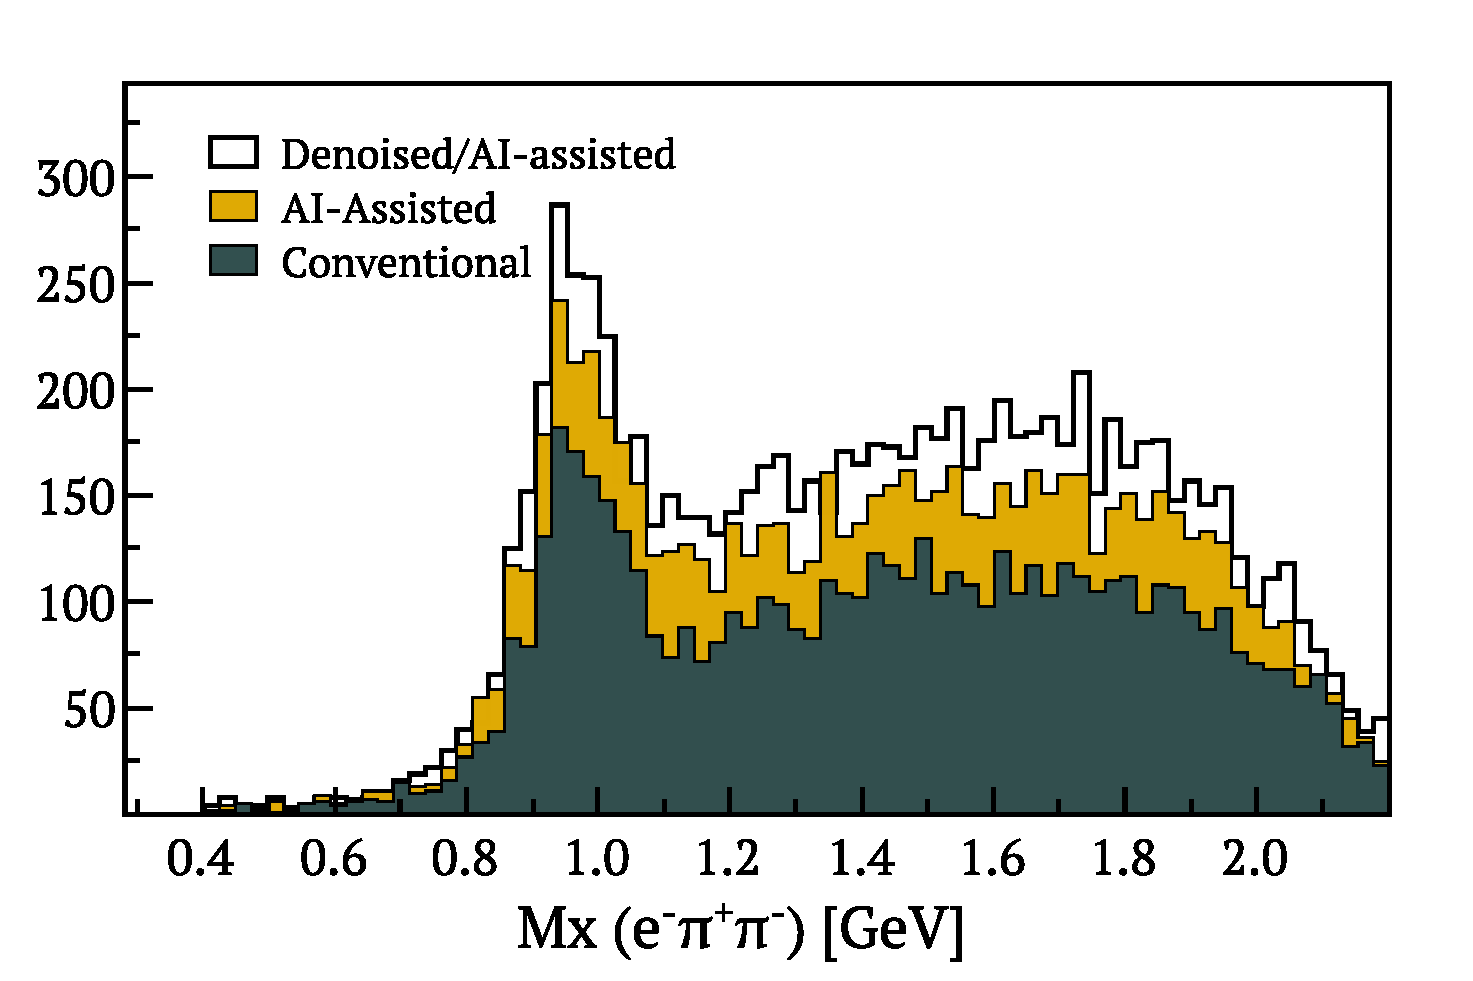
\includegraphics[width=0.44\columnwidth]{images/figure_denoise_mxp.pdf}
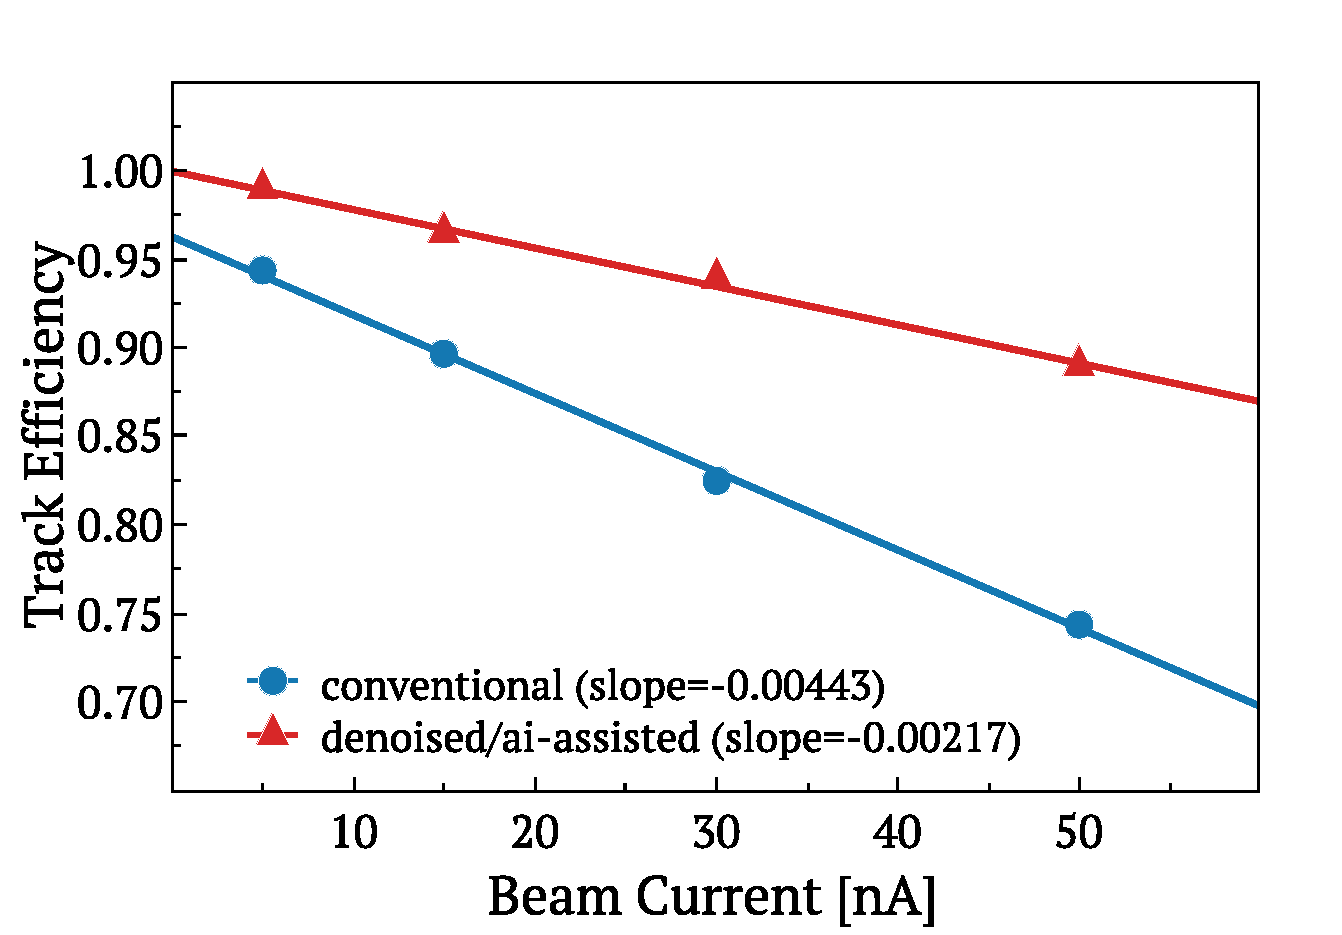
\includegraphics[width=0.42\columnwidth]{images/luminosity_scan.pdf}
\caption{The increase in statistics in the reaction $ep\rightarrow e^\prime\pi^+\pi^-(X)$ (left). The missing mass of three particles is plotted showing a peak for the missing proton for
three different workflows of reconstruction, "Conventional" is the tracking without interference from AI, "AI-Assisted" is track reconstruction where suggestions on track candidates are provided by AI classifier, and "Denoised/AI-Assisted" is where the raw data was first denoised by CAE and then tracks classifier finds track candidates and passed them to reconstruction procedure.  The dependence of the single-track reconstruction efficiency as a function of luminosity is compared for "Conventional" and "Denoised/AI-Assisted" workflows (right). } 
\label{fig:ai_vs_conv}
\end{figure}

In Figure~\ref{fig:ai_vs_conv}, the dependence of single particle reconstruction efficiency is shown as a function of luminosity (beam current), calculated from data taken at different beam currents. It is evident from the figure that using AI (Denoising and track-finding) significantly improves the efficiency loss as a function of luminosity, making it possible to run experiments at higher than design luminosities, leading to a significant increase in collected data for the experiments.

\section{Track Parameter Finding}

An Artificial Intelligence (AI) approach for track reconstruction was developed to estimate track parameters, such as momentum and direction, based on cluster positions along the track~\cite{Thomadakis:2023ebe}. The AI-estimated track parameters were shown to align more closely with those reconstructed using the Kalman filter compared to conventional hit-based tracking methods. This capability enables the identification of complete physics event topologies directly from raw hits in drift chambers, leveraging AI to achieve significantly faster processing than traditional tracking algorithms.

Figure~\ref{fig:ai_inference} presents the results of the track parameter predictions, demonstrating the accuracy of AI-reconstructed track parameters relative to the Kalman filter-based time-based tracking.

%Furthermore, an Artificial Intelligence approach to track reconstruction was developed to estimate track parameters 
%(such as momentum and direction) based on cluster positions of the track~\cite{Thomadakis:2023ebe}, it was shown that 
%the AI-estimated track parameters are closer to the values reconstructed using the Kalman-filter than the conventional hit-based tracking.
%This makes it possible to identify full physics event topologies from raw hits in drift chambers, using only Artificial Intelligence, much faster
%than conventional tracking algorithm. The results of track parameter predictions are shown in Figure~\ref{fig:ai_inference}, where the accuracy 
%track parameters reconstructed by AI are shown relative to Kalman-Filter-based Time-Based tracking is shown.

\begin{figure}[h!]
\centering
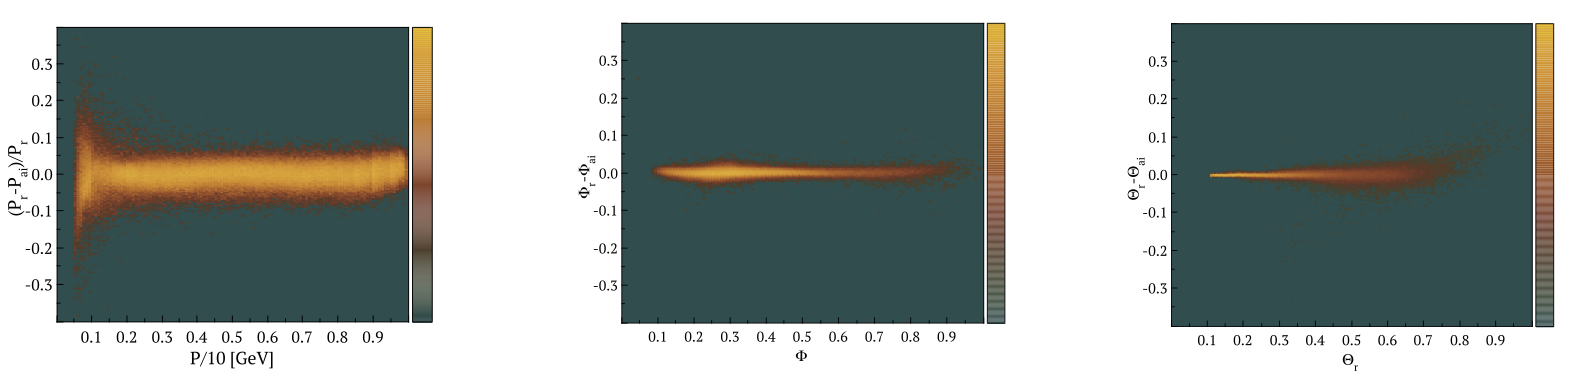
\includegraphics[width=0.85\columnwidth]{images/mlp_track_pars.png}
\caption{Results of track parameter estimating network (MLP) showing the difference between real track parameters and inferred parameters, for momentum, polar angle ($\theta$) and azimuthal angle ($\phi$). } 
\label{fig:ai_inference}
\end{figure}

Using track parameters predicted by AI, physics events can be analyzed to reconstruct particle final states. In Figure~\ref{fig:ai_instarec}, reconstructed particles are shown for two inclusive reactions, $ep\rightarrow e^\prime p K^- (K+)$ and $ep\rightarrow e^\prime\pi^+\pi^-(p)$, where cut on the missing mass of the system is placed around the mass of the missing particle. The peaks corresponding to $\Lambda^\circ (1520)$ and $\rho^\circ (770)$ can be seen in the figure.

\begin{figure}[h!]
\centering
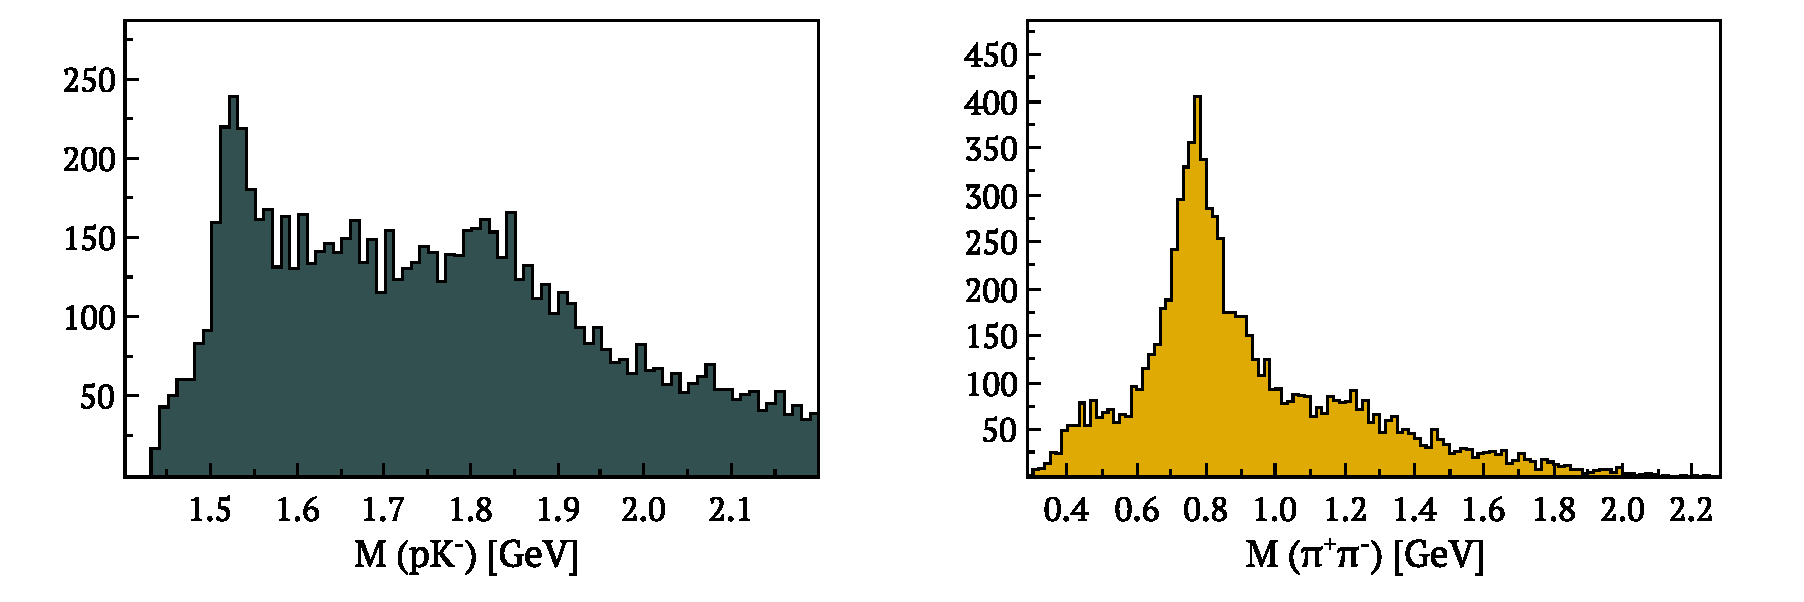
\includegraphics[width=0.85\columnwidth]{images/figure_lambda_instarec.pdf}
\caption{Particle reconstruction using the invariant mass of detected decay products for reactions $ep\rightarrow e^\prime p K^- (K+)$ and $ep\rightarrow e^\prime\pi^+\pi^-(p)$ respectively. The particle parameters used in calculating the invariant masses are derived by a neural network. A cut on missing mass was used to select appropriate exclusive reactions.} 
\label{fig:ai_instarec}
\end{figure}

The particle parameters, such as momentum and direction, in the physics distributions are derived from AI-based track reconstruction. However, the data files had to first undergo conventional reconstruction to select events containing the required particles, as particle species identification has not yet been integrated into the AI workflow. While our group has developed an electron identification system, it has not yet been incorporated into the AI tracking process. An ongoing project aims to enable full particle identification using AI. Once this capability is developed and implemented, it will be possible to generate such distributions in real-time during the data acquisition stage.

%The particle parameters (momentum and direction) in the physics distributions are taken from AI track reconstruction. However, the files had to be processed through the conventional reconstruction first to select the event with the required particles because we do not yet have particle species identification in the AI workflow. The electron identification has been 
%developed by our group, but it's not yet integrated into the AI tracking workflow, and there is an ongoing project for full particle identification using AI. Once the particle identification is 
%developed and implemented it will be possible to obtain such distributions in real-time during the data acquisition stage.

\section{Discussion}
In CLAS12, we have implemented robust AI support for track reconstruction, which is now actively used in production. This innovation has resulted in a significant improvement in statistics, with increases of $60\%–70\%$ depending on the physics reaction and event topology. Additionally, the AI-assisted track finding has enhanced the performance of conventional tracking code, delivering a $30\%$ speedup.

A comprehensive track reconstruction framework was developed to identify tracks directly from raw hits in drift chambers and predict track parameters with greater accuracy than traditional hit-based Kalman-filter fits. Benchmark testing demonstrated that the AI reconstruction operates at 8 kHz in a single-threaded mode, enabling multi-threaded deployment for online use. This approach can process physics events faster than the current CLAS12 data acquisition rate of 16–20 kHz.

The fast AI reconstruction will also be employed online to classify events by topology and organize them within the output data stream, significantly accelerating calibration and physics validation workflows. With the integration of electron identification neural networks, this system can function as a level-3 software trigger, enhancing the level-1 trigger purity and potentially reducing the data volume by up to $40\%$.

This development is a critical step toward enabling CLAS12's transition to streaming readout systems, where software-driven triggers are essential for reducing streaming data. Real-time tracking reconstruction and particle identification will be indispensable solutions in this new paradigm.

%In CLAS12, we developed strong AI support for our track reconstruction, which is currently used in production mode and results in a significant increase in statistics ($60\%-70\%$ depending on physics reaction and event topology). The AI-assisted track finding also resulted in a $30\%$ speedup of conventional tracking code. A full-track reconstruction framework was developed that can identify tracks from raw hits in drift chambers and predict the track parameters with accuracy better than hit-based Kalman-filter fit. The AI reconstruction was benchmarked to work at $8 kHz$ in a single thread, which makes it possible to deploy it online when multi-threaded and will be able to reconstruct physics events faster than CLAS12 data acquisition (currently at $16-20 kHz$). 
%The fast AI reconstruction will be used online to tag events by topology and sort them in the output data stream, which will significantly improve the data processing times for calibration
%and physics validation workflows. Furthermore, with the inclusion of electron identification neural networks, it can also serve as a level-3 software trigger to improve the purity of the level-1 trigger and potentially reduce the data by $40\%$. 
%This development will aid CLAS12 in the transition to streaming readout, where software-driven triggers are necessary to reduce the streaming data, and tracking reconstruction and particle identification in real-time is the only feasible solution.

\section{Acknowledgments}
This material is based upon work supported by the U.S. Department of Energy, Office of Science, Office of Nuclear Physics under contract DE-AC05-06OR23177, and NSF grant no. CCF-1439079 and the Richard T. Cheng Endowment. 
 
 
 \begin{thebibliography}{}
 \bibitem{Burkert:2020akg}
Burkert, V.D. and others, The CLAS12 Spectrometer at Jefferson Laboratory, Nucl. Instrum. Meth. A \textbf{959},163419 (2020)
% Format for Journal Reference
%Journal Author, Journal \textbf{Volume}, page numbers (year)
% Format for books
\bibitem{Mestayer:2020saf}
 "Mestayer, M.D. and others", The CLAS12 drift chamber system, Nucl. Instrum. Meth. A",\textbf{959} 163518 (2020)
\bibitem{Kalman1960}
  Kalman, R. E., A New Approach to Linear Filtering and Prediction Problems, Journal of Basic Engineering, \textbf{82}, 35-45 (1960)
\bibitem{Gavalian:2020oxg}
Gavalian, Gagik and Thomadakis, Polykarpos and Angelopoulos, Angelos and Ziegler, Veronique and Chrisochoides, Nikos, Using Artificial Intelligence for Particle Track Identification in CLAS12 Detector, \textbf{2008.12860}, (2020)
\bibitem{Gavalian:2020xmc}
 Gavalian Gagik,Auto-encoders for Track Reconstruction in Drift Chambers for CLAS12, \textbf{2009.05144}, (2020)
\bibitem{Thomadakis:2022zcd}
   Thomadakis, Polykarpos and Angelopoulos, Angelos and Gavalian, Gagik and Chrisochoides, Nikos, De-noising drift chambers in CLAS12 using convolutional autoencoders, \textbf{271}, 108201 (2022)   
   %\cite{Thomadakis:2023ebe}
\bibitem{Thomadakis:2023ebe} 
P.~Thomadakis, K.~Garner, G.~Gavalian and N.~Chrisochoides,
``Charged particle reconstruction in CLAS12 using Machine Learning,''
Comput. Phys. Commun. \textbf{287}, 108694 (2023) doi:10.1016/j.cpc.2023.108694
%2 citations counted in INSPIRE as of 06 Feb 2024
\bibitem{Gavalian:hipo} 
  G.Gavalian, High-Performance Output (HIPO) Data Format for CLAS12,  "https://github.com/gavalian/hipo"
%\bibitem{RefB}
%Book Author, \textit{Book title} (Publisher, place, year) page numbers
% etc
\end{thebibliography}
 
%\newpage
%\bibliography{references}
%\bibliographystyle{ieeetr}

\end{document}
